% !TeX TS-program = pdflatex


\documentclass[a4paper]{article}

% \usepackage[default]{fontsetup}

\usepackage{fancyhdr}
\usepackage{extramarks}
\usepackage{amsmath}
\usepackage{amsthm}
\usepackage{amsfonts}
\usepackage{tikz}
\usepackage[plain]{algorithm}
\usepackage{algpseudocode}
\usepackage{enumerate}
\usepackage{tikz}
\usepackage{amssymb}
\usepackage{amsfonts}
\usepackage{fdsymbol}



\usetikzlibrary{automata,positioning}

%
% Basic Document Settings
%  

\topmargin=-0.2in
\evensidemargin=0in
\oddsidemargin=0in
\textwidth=6.5in
\textheight=9.5in
\headsep=0.25in

\linespread{1.1}

\pagestyle{fancy}
\lhead{\hmwkAuthorName}
\chead{\hmwkClass : \hmwkTitle}
\rhead{\firstxmark}
\lfoot{\lastxmark}
\cfoot{\thepage}

\renewcommand\headrulewidth{0.4pt}
\renewcommand\footrulewidth{0.4pt}

\setlength\parindent{0pt}

%
% Create Problem Sections
%

\newcommand{\enterProblemHeader}[1]{
    \nobreak\extramarks{}{Problem \arabic{#1} continued on next page\ldots}\nobreak{}
    \nobreak\extramarks{Problem \arabic{#1} (continued)}{Problem \arabic{#1} continued on next page\ldots}\nobreak{}
}

\newcommand{\exitProblemHeader}[1]{
    \nobreak\extramarks{Problem \arabic{#1} (continued)}{Problem \arabic{#1} continued on next page\ldots}\nobreak{}
    \stepcounter{#1}
    \nobreak\extramarks{Problem \arabic{#1}}{}\nobreak{}
}

\newcommand*\circled[1]{\tikz[baseline=(char.base)]{
		\node[shape=circle,draw,inner sep=2pt] (char) {#1};}}


\setcounter{secnumdepth}{0}
\newcounter{partCounter}
\newcounter{homeworkProblemCounter}
\setcounter{homeworkProblemCounter}{1}
\nobreak\extramarks{Problem \arabic{homeworkProblemCounter}}{}\nobreak{}

%
% Homework Problem Environment
%
% This environment takes an optional argument. When given, it will adjust the
% problem counter. This is useful for when the problems given for your
% assignment aren't sequential. See the last 3 problems of this template for an
% example.
%

\newenvironment{homeworkProblem}[1][-1]{
    \ifnum#1>0
        \setcounter{homeworkProblemCounter}{#1}
    \fi
    \section{Problem \arabic{homeworkProblemCounter}}
    \setcounter{partCounter}{1}
    \enterProblemHeader{homeworkProblemCounter}
}{
    \exitProblemHeader{homeworkProblemCounter}
}

%
% Homework Details
%   - Title
%   - Class
%   - Due date
%   - Name
%   - Student ID

\newcommand{\hmwkTitle}{Homework\ \#07}
\newcommand{\hmwkClass}{Probability \& Statistics for EECS}
\newcommand{\hmwkDueDate}{2024-11-26}
\newcommand{\hmwkAuthorName}{Wenye Xiong}
\newcommand{\hmwkAuthorID}{2023533141}


%
% Title Page
%

\title{
    \vspace{2in}
    \textmd{\textbf{\hmwkClass:\\  \hmwkTitle}}\\
    \normalsize\vspace{0.1in}\small{Due\ on\ \hmwkDueDate\ at 23:59}\\
	\vspace{4in}
}

\author{
	Name: \textbf{\hmwkAuthorName} \\
	Student ID: \hmwkAuthorID}
\date{}

\renewcommand{\part}[1]{\textbf{\large Part \Alph{partCounter}}\stepcounter{partCounter}\\}

%
% Various Helper Commands
%

% Useful for algorithms
\newcommand{\alg}[1]{\textsc{\bfseries \footnotesize #1}}
% For derivatives
\newcommand{\deriv}[1]{\frac{\mathrm{d}}{\mathrm{d}x} (#1)}
% For partial derivatives
\newcommand{\pderiv}[2]{\frac{\partial}{\partial #1} (#2)}
% Integral dx
\newcommand{\dx}{\mathrm{d}x}
% Alias for the Solution section header
\newcommand{\solution}{\textbf{\large Solution}}
% Probability commands: Expectation, Variance, Covariance, Bias
\newcommand{\E}{\mathrm{E}}
\newcommand{\Var}{\mathrm{Var}}
\newcommand{\Cov}{\mathrm{Cov}}
\newcommand{\Bias}{\mathrm{Bias}}

\begin{document}


% \maketitle
% \thispagestyle{empty}
% \pagebreak

\date{
Due on Nov. 26, 2024, 11:59 UTC+8}
\title{SI 140A-02  Probability \& Statistics for EECS, Fall 2024 \\
Homework 7}
\maketitle
Read all the instructions below carefully before you start working on the assignment, and before you make a submission.
\begin{itemize}
    \item You are required to write down all the major steps towards making your conclusions; otherwise you may obtain limited points of the problem.
    \item Write your homework in English; otherwise you will get no points of this homework.
    \item Any form of plagiarism will lead to $0$ point of this homework. 
\end{itemize}
\newpage

\begin{homeworkProblem}[1]
\begin{enumerate}[(a)]
    \item Show the proof of general Bayes’ Rule (four cases).

\begin{figure}[H]
	\centering
	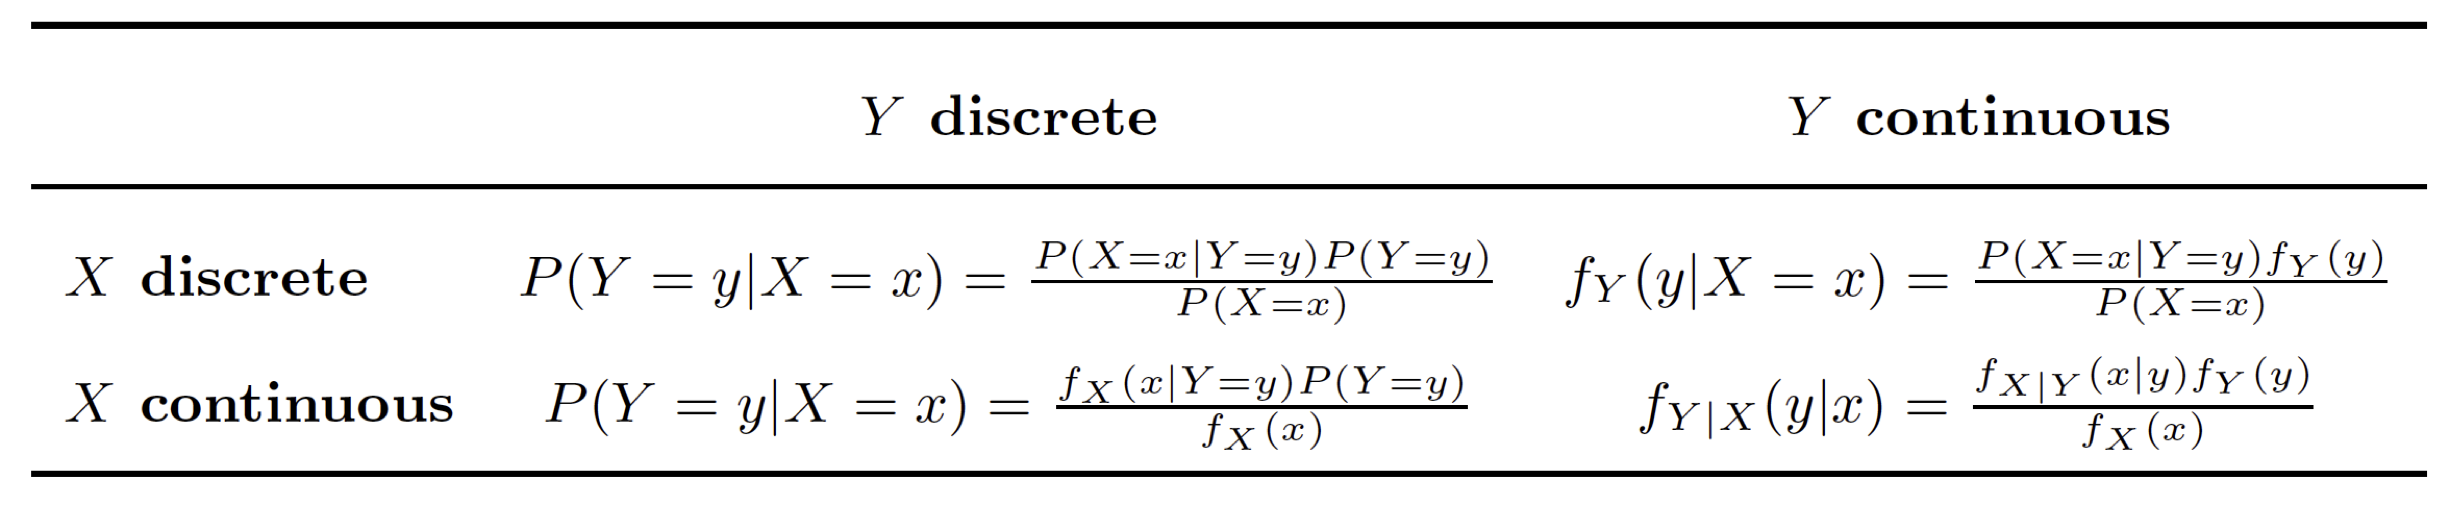
\includegraphics[scale=0.4]{figures/bayes.png}
\end{figure}

    \item Show the proof of general LOTP (four cases).

\begin{figure}[H]
	\centering
	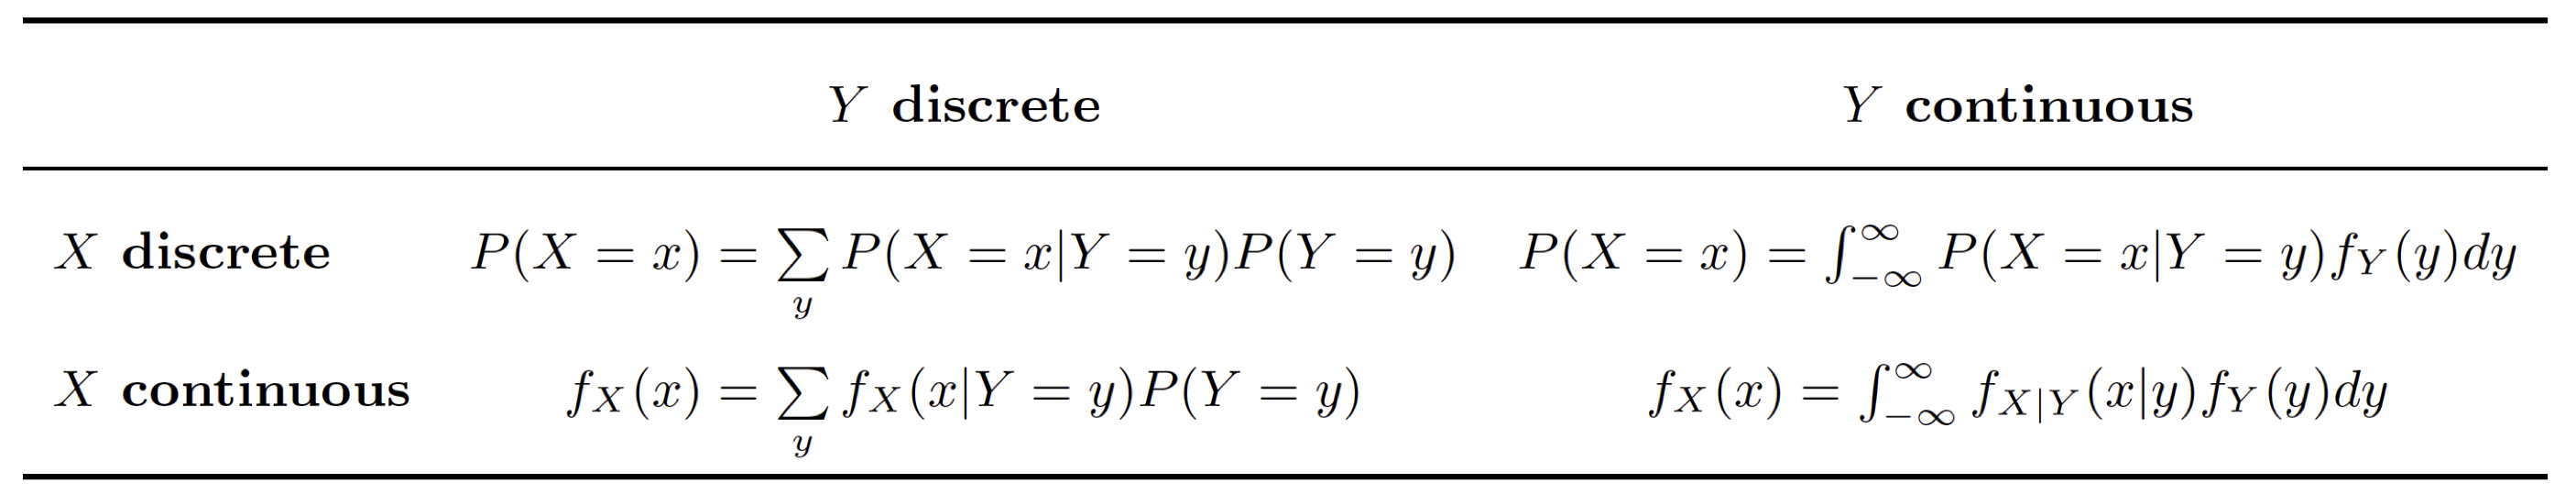
\includegraphics[scale=0.35]{figures/lotp.png}
\end{figure}

\end{enumerate}

\subsection{Solution}
(a):\\
If X is discrete, Y is continuous, then\\
According to the continuous Bayes' Rule, we have
\begin{center}
    $P(Y \in (y - \epsilon, y + \epsilon) | X = x) = \frac{P(X = x | Y \in (y - \epsilon, y + \epsilon))P(Y \in (y - \epsilon, y + \epsilon))}{P(X = x)}$
\end{center}
Let $\epsilon \to 0$, we have
\begin{center}
    $lim_{\epsilon \to 0} P(Y \in (y - \epsilon, y + \epsilon) | X = x) = lim_{\epsilon \to 0} f_Y(y | X = x) \cdot 2\epsilon $\\
    and \\
    $lim_{\epsilon \to 0} \frac{P(X = x | Y \in (y - \epsilon, y + \epsilon))P(Y \in (y - \epsilon, y + \epsilon))}{P(X = x)} = lim_{\epsilon \to 0} \frac{P(X = x | Y = y) f_Y(y) \cdot 2\epsilon}{P(X = x)}$
\end{center}
Thus, we have
\begin{center}
    $f_Y(y | X = x) = \frac{f_{X|Y}(x | y) f_Y(y)}{f_X(x)}$
\end{center}
If X is continuous, Y is discrete, then similarly, we have 
\begin{center}
    $P(Y = y | X = x) = lim_{\epsilon \to 0} P(Y = y | X \in (x - \epsilon, x + \epsilon)) = lim_{\epsilon \to 0} \frac{P(X \in (x - \epsilon, x + \epsilon) | Y = y)P(Y = y)}{P(X \in (x - \epsilon, x + \epsilon))}$\\
    $= lim_{\epsilon \to 0} \frac{f_X(x | Y = y) P(Y = y) \cdot 2\epsilon}{f_X(x) \cdot 2\epsilon} = \frac{f_X(x | Y = y) P(Y = y)}{f_X(x)}$
\end{center}
If X and Y are both discrete, this is just the simple Bayes' Rule.\\
Samely, if X and Y are both continuous, this is just the continuous Bayes' Rule.\\
(b):\\
If $X$ discrete, $Y$ continuous:
$$
P(X=x \mid Y \in(y-\varepsilon, y+\varepsilon))=\frac{P(Y \in(y-\varepsilon, y+\varepsilon) \mid X=x) P(X=x)}{P(Y \in(y-\varepsilon, y+\varepsilon))} .
$$

By letting $\varepsilon \rightarrow 0$, we have
$$
\lim _{\varepsilon \rightarrow 0} P(X=x \mid Y \in(y-\varepsilon, y+\varepsilon))=P(X=x \mid Y=y),
$$
and
$$
\begin{aligned}
& \lim _{\varepsilon \rightarrow 0} \frac{P(Y \in(y-\varepsilon, y+\varepsilon) \mid X=x) P(X=x)}{P(Y \in(y-\varepsilon, y+\varepsilon))} \\
= & \lim _{\varepsilon \rightarrow 0} \frac{f_Y(y \mid X=x) \cdot 2 \varepsilon \cdot P(X=x)}{f_Y(y) \cdot 2 \varepsilon} \\
= & \frac{f_Y(y \mid X=x) P(X=x)}{f_Y(y)} .
\end{aligned}
$$

By combining the two equations, we can get
$$
\begin{array}{r}
P(X=x \mid Y=y)=\frac{f_Y(y \mid X=x) P(X=x)}{f_Y(y)} \\
\Rightarrow P(X=x \mid Y=y) f_Y(y)=f_Y(y \mid X=x) P(X=x)
\end{array}
$$

By integrating on both sides of the equation with respect $y$, we can get
$$
\begin{aligned}
\int_{-\infty}^{\infty} P(X=x \mid Y=y) f_Y(y) d y & =\int_{-\infty}^{\infty} f_Y(y \mid X=x) P(X=x) d y \\
& =P(X=x) \int_{-\infty}^{\infty} f_Y(y \mid X=x) d y \\
& =P(X=x)
\end{aligned}
$$
If $X$ continuous, $Y$ discrete:
$$
P(X \in(x-\varepsilon, x+\varepsilon))=\sum_y P(X \in(x-\varepsilon, x+\varepsilon) \mid Y=y) P(Y=y) .
$$

Let $\varepsilon \rightarrow 0$, we have
$$
\lim _{\varepsilon \rightarrow 0} P(X \in(x-\varepsilon, x+\varepsilon))=\lim _{\varepsilon \rightarrow 0} f_X(x) \cdot 2 \varepsilon
$$
and
$$
\lim _{\varepsilon \rightarrow 0} \sum_y P(X \in(x-\varepsilon, x+\varepsilon) \mid Y=y) P(Y=y)=\lim _{\varepsilon \rightarrow 0} \sum_y f_X(x \mid Y=y) \cdot 2 \varepsilon \cdot P(Y=y) .
$$

Combining the two equations, we get
$$
\begin{gathered}
\lim _{\varepsilon \rightarrow 0} f_X(x) \cdot 2 \varepsilon=\lim _{\varepsilon \rightarrow 0} \sum_y f_X(x \mid Y=y) \cdot 2 \varepsilon \cdot P(Y=y) \\
f_X(x)=\sum_y f_X(x \mid Y=y) P(Y=y)
\end{gathered}
$$

The situation of $X$ and $Y$ both discrete is just the simple LOTP.\\
The situation of $X$ and $Y$ both continuous is just the continuous LOTP.\\
\end{homeworkProblem}
\newpage

\begin{homeworkProblem}[2]
A chicken lays a $\text{Pois}(\lambda)$ number $N$ of eggs.
	Each egg hatches a chick with probability $p$, independently.
	Let $X$ be the number which hatch, and $Y$ be the number which do NOT hatch.
	
\begin{enumerate}[(a)]
    \item
    Find the joint PMF of $N, X, Y$.
    Are they independent?
    
    \item
    Find the joint PMF of $N, X$.
    Are they independent?
    
    \item
    Find the joint PMF of $X, Y$.
    Are they independent?
    
    \item
    Find the correlation between $N$ (the number of eggs) and $X$ (the number of eggs which hatch).
    Simplify; your final answer should work out to a simple function of $p$ (the $\lambda$ should cancel out).
\end{enumerate}
\subsection{Solution}
We can easily get that $X$ is distributed $\operatorname{Pois}(p \lambda)$ and $Y$ similarly $\operatorname{Pois}(q \lambda)$ with $q=1-p$ and these random variables are independent.
\\
(a) \\
For non-negative integer $i, j, n$, if $i+j \neq n, P(X=i, Y=j, N=n)=0$.

If $i+j=n$, then
$$
P(X=i, Y=j, N=n)=P(X=i, Y=j \mid N=n) P(N=n)=\binom{n}{i} p^i q^{n-i} \cdot \frac{\lambda^n}{n!} e^{-\lambda} .
$$
$X, Y$, and $N$ are not independent because we have that for $i, j, n>0$ such that $i+j \neq n$
$$
P(X=i, Y=j, N=n)=0 .
$$

But obviously we have that
$$
P(X=i) P(Y=j) P(N=n)>0 \text {. }
$$\\
(b)\\
 For $n \geq i \geq 0$,
$$
P(X=i, N=n)=P(X=i \mid N=n) P(N=n)=\binom{n}{i} p^i q^{n-i} \cdot \frac{\lambda^n}{n!} e^{-\lambda}, n \geq i \geq 0
$$

Otherwise, $P(X=i, N=n)=0$.
$X$ and $N$ are not independent since from the story, $X \sim \operatorname{Pois}(p \lambda)$, then we have
$$
P(X=i) P(N=n)=\frac{(\lambda p)^i}{i!} e^{-\lambda p} \cdot \frac{\lambda^n}{n!} e^{-\lambda}
$$
which is obviously not equal to the joint PMF. 
\\(c) \\
$X$ and $Y$ are independent, so the joint distribution is
$$
P(X=i, Y=j)=P(X=i) P(Y=j)=\frac{(\lambda p)^i}{i!} e^{-\lambda p} \frac{(\lambda q)^j}{j!} e^{-\lambda q}, i, j \geq 0 .
$$\\
(d) \\By the property of covariance,
$$
\operatorname{Cov}(N, X)=\operatorname{Cov}(X+Y, X)=\operatorname{Cov}(X, X)+\operatorname{Cov}(X, Y)=\operatorname{Var}(X)=\lambda p
$$

Since $N \sim \operatorname{Pois}(\lambda), \operatorname{Var}(N)=\lambda$, we have
$$
\operatorname{Corr}(N, X)=\frac{\operatorname{Cov}(N, X)}{\sqrt{\operatorname{Var}(N) \operatorname{Var}(X)}}=\frac{\lambda p}{\sqrt{\lambda \cdot \lambda p}}=\sqrt{p}
$$
\end{homeworkProblem}

\newpage
\begin{homeworkProblem}[3]
Let $X$ and $Y$ be i.i.d. $\operatorname{Expo}(\lambda)$, and $T=X+Y$.
	
\begin{enumerate}[(a)]
	\item  Find the conditional CDF of $T$ given $X=x$. Be sure to specify where it is zero.
	\item  Find the conditional PDF $f_{T \mid X}(t \mid x)$, and verify that it is a valid PDF.
	\item  Find the conditional PDF $f_{X \mid T}(x \mid t)$, and verify that it is a valid PDF.
	\item In class we have shown that the marginal PDF of $T$ is $f_{T}(t)=\lambda^{2} t e^{-\lambda t}$, for $t>0 .$ Give a short alternative proof of this fact, based on the previous parts and Bayes' rule.
\end{enumerate}

\subsection{Solution}
(a)\\
$$
F_{T \mid X}(t \mid x)=P(T \leq t \mid X=x)=P(X+Y \leq t \mid X=x)=P(Y \leq t-x)=\left(1-e^{-\lambda(t-x)}\right) \cdot \chi_{t \geq x} .
$$
(b) \\
We take derivative from $F_{T \mid X}$ respective to $t$.
$$
f_{T \mid X}(t \mid x)=\frac{\partial}{\partial t} F_{T \mid X}(t \mid x)=\frac{\partial}{\partial t}\left[\left(1-e^{-\lambda(t-x)}\right) \cdot \chi_{t \geq x}\right]=\lambda e^{-\lambda(t-x)} \cdot \chi_{t \geq x} .
$$
$$
f_{T \mid X}(t \mid x)=\lambda e^{-\lambda(t-x)} \cdot \chi_{t \geq x}= \begin{cases}0 \geq 0, & t<x \\ \lambda e^{-\lambda(t-x)} \geq 0, & t \geq x\end{cases}
$$
This shows that $f_{T \mid X}(t \mid x)$ is non-negative.\\
$$
\int_{-\infty}^{\infty} f_{T \mid X}(t \mid x) d t=\int_x^{\infty} \lambda e^{-\lambda(t-x)} d t=-\left.e^{-\lambda(t-x)}\right|_{t=x} ^{t=\infty}=1
$$
This shows that $f_{T \mid X}(t \mid x)$ integrates to 1.\\
Therefore, $f_{T \mid X}(t \mid x)$ is valid PDF.\\
(c)\\
$$
\begin{aligned}
f_{X \mid T}(x \mid t) & =\frac{f_{T \mid X}(t \mid x) f_X(x)}{f_T(t)} \\
& =\frac{1}{f_T(t)} \lambda e^{-\lambda(t-x)} \cdot \lambda e^{-\lambda x} \cdot \chi_{t \geq x} \\
& =\frac{1}{f_T(t)} \lambda^2 e^{-\lambda t} \cdot \chi_{t \geq x}
\end{aligned}
$$
$$
f_{X \mid T}(x \mid t)=\frac{1}{f_T(t)} \lambda^2 e^{-\lambda t} \cdot \chi_{t \geq x}= \begin{cases}0 \geq 0, & t<x \\ \frac{1}{f_T(t)} \lambda^2 e^{-\lambda t} \geq 0, & t \geq x\end{cases}
$$
This shows that $f_{X \mid T}(x \mid t)$ is non-negative.\\
Note that $f_{X \mid T}(x \mid t)=\frac{1}{f_T(t)} \lambda^2 e^{-\lambda t} \cdot \chi_{t \geq x}$ is constant with respect to $x$. In particular, $f_{X \mid T}(x \mid t)$ is a non-zero constant respect to $x$ over support $(0, t)$ and zero otherwise. By definition of Uniform distribution, we have $X \mid T=t \sim \operatorname{Unif}(0, t)$, hence a valid PDF $f_{X \mid T}(x \mid t)$ over support $(0, t)$.
\\
(d) \\
According to (c), $X | T = t \sim \operatorname{Unif}(0, t)$, so $f_{X | T}(x | t) = \frac{1}{t} \chi_{0 \leq x \leq t}$.\\
According to Bayes' Rule, we have
$$
f_{T}(t)=\frac{f_{X | T}(t | x) f_X(x)}{f_{X | T}(x | t)}=\frac{\lambda^2 e^{-\lambda t} \chi_{0 \leq x \leq t}}{\frac{1}{t}\chi_{0 \leq x \leq t}}=\lambda^2 t e^{-\lambda t} 
$$
\end{homeworkProblem}

\newpage
\begin{homeworkProblem}[4]
Let $U_1, U_2, U_3$ be i.i.d. Unif$(0,1)$, and let $L = \min(U_1,U_2,U_3)$, $M = \max(U_1, U_2, U_3)$.
\begin{enumerate}[(a)]
    \item Find the marginal CDF and marginal PDF of $M$, and the joint CDF and joint PDF of $L,M$. \\
    Hint: For the latter, start by considering $P(L \ge l,M \le m)$.
    \item  Find the conditional PDF of $M$ given $L$.
\end{enumerate}

\subsection{Solution}
(a) \\
Event $M \leq m$ is the same as the event that all 3 of the $U_j$ are at most $m$, so the CDF of $M$ is $F_M(m)=m^3$ and the PDF is $f_M(m)=3 m^2$, for $0 \leq m \leq 1$. \\
Event $L \geq l, M \leq m$ is the same as the event that all 3 of the $U_j$ are between $l$ and $m$ (inclusive), so
$$
P(L \geq l, M \leq m)=(m-l)^3
$$
for $m \geq l$ with $m, l \in[0,1]$. By the axioms of probability, we have
$$
P(M \leq m)=P(L \leq l, M \leq m)+P(L>l, M \leq m)
$$

So the joint CDF is
$$
P(L \leq l, M \leq m)=m^3-(m-l)^3,
$$
for $m \geq l$ with $m, l \in[0,1]$. The joint PDF is obtained by differentiating this with respect to $l$ and then with respect to $m$ (or vice versa):
$$
f(l, m)=6(m-l)
$$
for $m \geq l$ with $m, l \in[0,1]$. \\
(b) \\
The marginal PDF of $L$ is $f_L(l)=3(1-l)^2$ for $0 \leq l \leq 1$ since $P(L>l)=P\left(U_1>l, U_2>l, U_3>\right.$ $l)=(1-l)^3$  So the conditional PDF of $M$ given $L$ is
$$
f_{m \mid L}(m \mid l)=\frac{f(l, m)}{f_L(l)}=\frac{2(m-1)}{(1-l)^2}
$$
for all $m, l \in[0,1]$ with $m \geq l$.
\end{homeworkProblem}

\newpage
\begin{homeworkProblem}[5]
This problem explores a visual interpretation of covariance. Data are collected for $n \geq$ 2 individuals, where for each individual two variables are measured (e.g., height and weight). Assume independence across individuals (e.g., person 1's variables gives no information about the other people), but not within individuals (e.g., a person's height and weight may be correlated). 

Let $\left(x_{1}, y_{1}\right), \ldots,\left(x_{n}, y_{n}\right)$ be the $n$ data points. The data are considered here as fixed, known numbers-they are the observed values after performing an experiment. Imagine plotting all the points $\left(x_{i}, y_{i}\right)$ in the plane, and drawing the rectangle determined by each pair of points. For example, the points $(1,3)$ and $(4,6)$ determine the rectangle with vertices $(1,3),(1,6),(4,6),(4,3)$.

The signed area contributed by $\left(x_{i}, y_{i}\right)$ and $\left(x_{j}, y_{j}\right)$ is the area of the rectangle they determine if the slope of the line between them is positive, and is the negative of the area of the rectangle they determine if the slope of the line between them is negative. (Define the signed area to be 0 if $x_{i}=x_{j}$ or $y_{i}=y_{j}$, since then the rectangle is degenerate.) So the signed area is positive if a higher $x$ value goes with a higher $y$ value for the pair of points, and negative otherwise. Assume that the $x_{i}$ are all distinct and the $y_{i}$ are all distinct.
\begin{enumerate}[(a)]
	\item The sample covariance of the data is defined to be
	$$
	r=\frac{1}{n} \sum_{i=1}^{n}\left(x_{i}-\bar{x}\right)\left(y_{i}-\bar{y}\right)
	$$
	where
	$$
	\bar{x}=\frac{1}{n} \sum_{i=1}^{n} x_{i} \text { and } \bar{y}=\frac{1}{n} \sum_{i=1}^{n} y_{i}
	$$
	are the sample means. (There are differing conventions about whether to divide by $n-1$ or $n$ in the definition of sample covariance, but that need not concern us for this problem.)
	
	Let $(X, Y)$ be one of the $\left(x_{i}, y_{i}\right)$ pairs, chosen uniformly at random. Determine precisely how $\operatorname{Cov}(X, Y)$ is related to the sample covariance.
	
	\item Let $(X, Y)$ be as in (a), and $(\tilde{X}, \tilde{Y})$ be an independent draw from the same distribution. That is, $(X, Y)$ and $(\tilde{X}, \tilde{Y})$ are randomly chosen from the $n$ points, independently (so it is possible for the same point to be chosen twice).
	
	Express the total signed area of the rectangles as a constant times $E((X-\tilde{X})(Y-\tilde{Y}))$. Then show that the sample covariance of the data is a constant times the total signed area of the rectangles.
	
	Hint: Consider $E((X-\tilde{X})(Y-\tilde{Y}))$ in two ways: as the average signed area of the random rectangle formed by $(X, Y)$ and $(\tilde{X}, \tilde{Y})$, and using properties of expectation to relate it to $\operatorname{Cov}(X, Y)$. For the former, consider the $n^{2}$ possibilities for which point $(X, Y)$ is and which point $(\tilde{X}, \tilde{Y})$; note that $n$ such choices result in degenerate rectangles.
	\item Based on the interpretation from (b), give intuitive explanations of why for any r.v.s $W_{1}, W_{2}, W_{3}$ and constants $a_{1}, a_{2}$, covariance has the following properties:
	
	(i) $\operatorname{Cov}\left(W_{1}, W_{2}\right)=\operatorname{Cov}\left(W_{2}, W_{1}\right)$;
	
	(ii) $\operatorname{Cov}\left(a_{1} W_{1}, a_{2} W_{2}\right)=a_{1} a_{2} \operatorname{Cov}\left(W_{1}, W_{2}\right)$;
	
	(iii) $\operatorname{Cov}\left(W_{1}+a_{1}, W_{2}+a_{2}\right)=\operatorname{Cov}\left(W_{1}, W_{2}\right) ;$
	
	(iv) $\operatorname{Cov}\left(W_{1}, W_{2}+W_{3}\right)=\operatorname{Cov}\left(W_{1}, W_{2}\right)+\operatorname{Cov}\left(W_{1}, W_{3}\right)$.
\end{enumerate}

\subsection{Solution}
(a)\\ Since $(X, Y)$ is chosen uniformly at random, we have
$$
\mathrm{E}(X)=\sum_{i=1}^n x_i P\left(X=x_i\right)=\frac{1}{n} \sum_{i=1}^n x_i=\bar{x} ; \quad \mathrm{E}(Y)=\sum_{i=1}^n y_i P\left(Y=y_i\right)=\frac{1}{n} \sum_{i=1}^n y_i=\bar{y}
$$

By definition, we know
$$
\begin{aligned}
\operatorname{Cov}(X, Y) & =\mathrm{E}[(X-\mathrm{E}(X))(Y-\mathrm{E}(Y))] \\
& =\sum_{i=1}^n\left(x_i-\mathrm{E}(X)\right)\left(y_i-\mathrm{E}(Y)\right) P\left(X=x_i, Y=y_i\right) \\
& =\frac{1}{n} \sum_{i=1}^n\left(x_i-\bar{x}\right)\left(y_i-\bar{y}\right)=r
\end{aligned}
$$

Thus we have proved that $\operatorname{Cov}(X, Y)$ equals the sample covariance $r$.\\

(b)\\  Denote the total signed area of the rectangles as $S$, then
$$
S=\sum_{i=1}^n \sum_{j=1}^n\left(x_i-x_j\right)\left(y_i-y_j\right)
$$

Since $(X, Y)$ and $(\tilde{X}, \tilde{Y})$ are independent, we have
$$
\begin{aligned}
\mathrm{E}((X-\tilde{X})(Y-\tilde{Y})) & =\sum_{i=1}^n \sum_{j=1}^n\left(x_i-x_j\right)\left(y_i-y_j\right) P\left(X=x_i, Y=y_i\right) P\left(\tilde{X}=x_j, \tilde{Y}=y_j\right) \\
& =\frac{1}{n^2} \sum_{i=1}^n \sum_{j=1}^n\left(x_i-x_j\right)\left(y_i-y_j\right)=\frac{S}{n^2}
\end{aligned}
$$

Thusly we have $S=n^2 \mathrm{E}((X-\tilde{X})(Y-\tilde{Y}))$.
- By the properties of expectation and considering that $(X, Y)$ and $(\tilde{X}, \tilde{Y})$ are identically and independently sampled, we have
$$
\begin{aligned}
\mathrm{E}((X-\tilde{X})(Y-\tilde{Y})) & =\mathrm{E}(X Y)-\mathrm{E}(\tilde{X} Y)-\mathrm{E}(X \tilde{Y})+\mathrm{E}(\tilde{X} \tilde{Y}) \\
& =\mathrm{E}(X Y)-\mathrm{E}(\tilde{X}) \mathrm{E}(Y)-\mathrm{E}(X) \mathrm{E}(\tilde{Y})+\mathrm{E}(\tilde{X} \tilde{Y}) \\
& =\mathrm{E}(X Y)-\mathrm{E}(X) \mathrm{E}(Y)-\mathrm{E}(\tilde{X}) \mathrm{E}(\tilde{Y})+\mathrm{E}(\tilde{X} \tilde{Y}) \\
& =2[\mathrm{E}(X Y)-\mathrm{E}(X) \mathrm{E}(Y)] \\
& =2 \operatorname{Cov}(X, Y)=2 r .
\end{aligned}
$$

Thusly we have $r=\frac{S}{2 n^2}$.\\
(c)\\  The claim (i) is true because it doesn't matter what is the base and what is the height of the rectangle, we can switch them.\\
- The claim (ii) is true because rescaling the one coordinate by the factor $c$ yields that the total area of the rectangle rescales for $c$.\\
- The claim (iii) is true since the area of the rectangle is invariant on linear translation.\\
- The claim (iv) is true because the distributive property of the area: it doesn't matter if we calculate two areas with the same base and then sum them or first we add heights and then calculate the total area.
\end{homeworkProblem}


\newpage
\begin{homeworkProblem}[6] (\textbf{Optional Challenging Problem})\\
We use the notation $X \Vbar Y \mid Z$ to represent the
statement: random variables $X$ and $Y$ are conditionally independent given random
variable $Z$. Now given any four continuous random variables $X, Y, Z, W$, show the
following properties of conditional independence:
\begin{enumerate}
    \item Symmetry:
   	\begin{equation*}
   		X \Vbar Y \mid Z \iff Y \Vbar X \mid Z.		
   	\end{equation*}
    \item Decomposition:
    \begin{equation*}
    	X \Vbar (Y, W) \mid Z \Rightarrow X \Vbar Y \mid Z.
    \end{equation*}
    \item Weak Union:
   	\begin{equation*}
   		X \Vbar (Y,W) \mid Z \Rightarrow X \Vbar (Y,W) \mid (Z,W).
   	\end{equation*}
    \item Contract:
    \begin{equation*}
    	X \Vbar Y \mid Z \ \& \ X \Vbar W \mid (Y,Z) \iff X \Vbar (Y,W) \mid Z.
    \end{equation*}
    \item Intersection: For any positive joint PDF of $X, Y, Z, W$, 
    \begin{equation*}
    	X \Vbar Y \mid (Z,W) \ \& \ X \Vbar Z \mid (Y,W) \iff X \Vbar (Y, Z) \mid W.
    \end{equation*}
\end{enumerate}

In fact, these properties are found by Judea Pearl, who won 2011 Turing Award for fundamental contributions to artificial intelligence through the development of a calculus for probabilistic and causal reasoning.
As Judea Pearl commented: ``Exploiting conditional independence to generate fast probabilistic computations is one of the main contributions CS has made to probability theory.''

\end{homeworkProblem}
\end{document}